\documentclass[]{article}

% Packages
\usepackage{import}
\usepackage{blindtext}
\usepackage[utf8]{inputenc}
\usepackage[T1]{fontenc}
\usepackage{wasysym}
\usepackage{enumerate}
\usepackage{hyperref}
\usepackage{graphicx}
\usepackage[table]{xcolor}
\renewcommand{\arraystretch}{1.5} % sets the hight of the table row relative to the default hight
\usepackage{listings}
\lstset{basicstyle=\ttfamily,
	showstringspaces=false,
	commentstyle=\color{red},
	keywordstyle=\color{blue}
}
\usepackage{caption}
\usepackage[letterpaper, margin=1in]{geometry}
\usepackage[final]{pdfpages}
\usepackage{graphicx}
\usepackage{subcaption}
\usepackage[english]{babel}
\usepackage{float}
\usepackage{wrapfig}
%\usepackage{natbib}
\usepackage[
backend=biber,
style=ieee,
citestyle=numeric 
]{biblatex}
\addbibresource{reportLab10Python.bib}
%\usepackage{minted}

\definecolor{mGreen}{rgb}{0,0.6,0}
\definecolor{mGray}{rgb}{0.5,0.5,0.5}
\definecolor{mPurple}{rgb}{0.58,0,0.82}
\definecolor{pred}{rgb}{0.58,0,0}
\definecolor{backgroundColour}{rgb}{0.95,0.95,0.92}
\definecolor{deepblue}{rgb}{0,0,0.5}
\definecolor{brightblue}{rgb}{0.51, 0.61, 0.93}
\definecolor{deepred}{rgb}{0.6,0,0}
\definecolor{deepgreen}{rgb}{0,0.5,0}

%
%\lstdefinestyle{CStyle}{
%	backgroundcolor=\color{backgroundColour},   
%	commentstyle=\color{mGreen},
%	keywordstyle=\color{magenta},
%	numberstyle=\tiny\color{mGray},
%	stringstyle=\color{mPurple},
%	basicstyle=\footnotesize,
%	breakatwhitespace=false,         
%	breaklines=true,                 
%	captionpos=b,                    
%	keepspaces=true,                 
%	numbers=left,                    
%	numbersep=5pt,                  
%	showspaces=false,                
%	showstringspaces=false,
%	showtabs=false,                  
%	tabsize=2,
%	language=C
%}
%
% Python style for highlighting
%\newcommand\pythonstyle{\lstset{
%		language=Python,
%		basicstyle=\ttm,
%		otherkeywords={self},             % Add keywords here
%		keywordstyle=\ttb\color{deepblue},
%		emph={MyClass,__init__},          % Custom highlighting
%		emphstyle=\ttb\color{deepred},    % Custom highlighting style
%		stringstyle=\color{deepgreen},
%		frame=tb,                         % Any extra options here
%		showstringspaces=false            % 
%		numbers=left,                    
%		numbersep=5pt,
%}}
\lstdefinestyle{PythonStyle}{
	backgroundcolor=\color{backgroundColour}, 
	basicstyle=\ttm,
	otherkeywords={self},   
	commentstyle=\color{brightblue},
	keywordstyle=\color{deepblue},
	numberstyle=\tiny\color{mGray},
	stringstyle=\color{pred},
	identifierstyle=\color{mGreen},
	emph={MyClass,__init__},          % Custom highlighting
	emphstyle=\color{deepred},
	basicstyle=\footnotesize,
	breakatwhitespace=false,         
	breaklines=true,                 
	captionpos=b,                    
	keepspaces=true,                 
	numbers=left,                    
	numbersep=5pt,                  
	showspaces=false,                
	showstringspaces=false,
	showtabs=false,                  
	tabsize=2,
	language=Python
}

% Title Page
\title{ 
\includegraphics[scale=0.2]{01_images/gvsu_logo_marktop_SEPCEC_K_R.png}
		\linebreak 	\linebreak \linebreak
		EGR680 High Level Implementation on FPGA
		\linebreak \linebreak 
		Laboratory 10
		\linebreak \linebreak 
		PYNQ Embedded Design using Jupyter Notebooks
		\linebreak \linebreak \linebreak
		Professor: Dr. C. Parikh
		}
\author{Student: Dimitri Häring } %\thanks{Thanks } }
\date{November 13, 2018}

\begin{document}
\maketitle
\thispagestyle{empty}
\newpage
%\begin{abstract}
%\end{abstract}

\tableofcontents
%\listoftables
\listoffigures
\lstlistoflistings

\pagebreak
% content
\section{Introduction}\label{sec: Introduction}
The goal of final project is to familiarize the student with the groove connector and the possible interface methods provided with MicroBlaze and low level C code. The student will also write a software pulse width modulation (PWM). The outlined tasks are build on the PYNQ platform shown in Figure \ref{fig: intro1}. The MicroBlaze system is placed in between of the peripherals and the Zynq processing system (PS) as shown in Figure \ref{fig: intro2}. The MicroBlaze is in fact an from Xilinx developed softcore.

\begin{figure}[H]
	\centering
	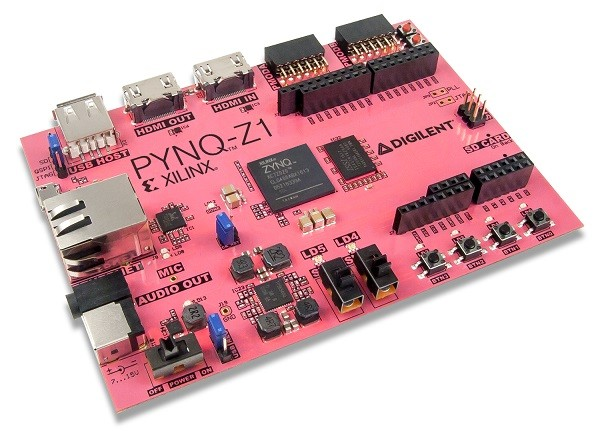
\includegraphics[width=0.6\textwidth]{01_images/PYNQ_Hardware_Xilinx}
	\caption{Xilinx PYNQ-Z1 development board SoC \cite{XUP}.}
	\label{fig: intro1}
\end{figure}
\begin{figure}[H]
	\centering
	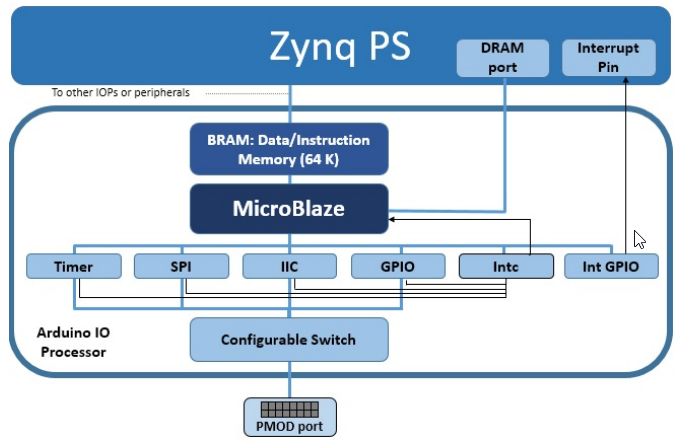
\includegraphics[width=0.8\textwidth]{01_images/PYNQ_Microblaze_Subsystem_Block_Diagram}
	\caption{PYNQ-Z1 block diagram of the MicroBlaze subsystem \cite{pynq_dr}.}
	\label{fig: intro2}
\end{figure}


\section{Design}\label{sec: Design}
In this section the design and decisions that where made to achieve it are discussed.

\subsection{Part 1 - Behavioral Modeling of a Seven-Segment Display}\label{sub: Behavioral Modeling of a Seven-Segment Display}
Verilog is used to describe a decoder that shall control a seven-segment display with two switches and one button. The given task is as followed:
\\
In this part, you will simulate a pattern decoder using the buttons, switches, and a single seven-segment display.
Using switches, SW0 and SW1 as the pattern input, write a Verilog program that takes the binary input
combinations of the switches and displays the decimal value of the binary switch combination on the seven-segment
display. Table 1 shows the switch combinations with the expected output value on the seven-segment
display.

\begin{figure}[htbp]
	\centering
	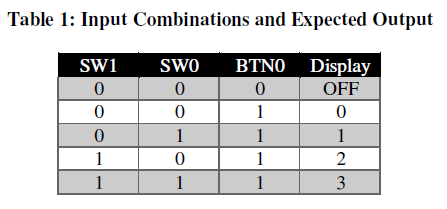
\includegraphics[width=0.6\textwidth]{01_images/Vivado_lab2_part1_table1.png}
	%\caption{Schematic directional coupler \cite{Vizmuller1995}}
	\label{fig: Vivado_lab2_part1_table1}
\end{figure}

As software package to implement the decoder in Verilog Vivado 2017.2 is used. 

%
%The maximum current of the directional coupler can be calculated as follow

%
%The used schematic is shown in figure \ref{fig: Schematic directional coupler} which is based on two transformers T1 and T2.
%
%\begin{figure}[htbp]
%	\centering
%	\includegraphics[width=\textwidth]{images/RFDG_p107_Coupler_Schematic.jpg}
%	\caption{Schematic directional coupler \cite{Vizmuller1995}}
%	\label{fig: Schematic directional coupler}
%\end{figure}
%
%As design a multi core ferrite made of Material 67 was chosen as basis to wind the coupler.
%\begin{itemize}
% \item \begin{description}
% 	\item [Mfr.:] Fair-Rite
% 	\item [Mfr. \#:] 2867000102
% 	\item [Description] Ferrite Toroids / Ferrite Rings 67 MULIT APERTURE 13.3mm 13.4mm 7.5mm
% \end{description}
%\end{itemize}
%The wire used to wrap the coupler is AWG 22 magnet wire. According to tables on the Internet there is a current rating range from 0.9 A up to 5 A, so it is not unreasonable to not assume that it will be ok to operate the coupler on 50 W power.
%\begin{itemize}
%	\item \begin{description}
%	\item[Mfr.:] CNC Tech
%	\item[Mfr. \#:] 600222
%	\item [Description] MW35-C HY 22AWG 1KG/2.2LBS SPOOL
%	\item [Digi-Key Part Number]	1175-1687-ND	
%\end{description}
%\end{itemize}
%
%From the the Fair-Rite web page following information is available shown in figure \ref{fig: 67 Material Ferrite Toroid } which shows the complex permeability vs frequency and permeability vs temperature.
%
%\begin{figure}[htbp]
%	\centering
%	\begin{subfigure}[b]{0.4\textwidth}
%		\centering
%		\includegraphics[width=\textwidth ]{images/Ferrite-Torroit-67-Perm-vs-Freq2.jpg}
%		\caption{67 Material Characteristics}
%	\end{subfigure}
%	\begin{subfigure}[b]{0.4\textwidth}
%		\centering
%		\includegraphics[width=\textwidth]{images/Ferrite-Torroit-67-Perm-vs-Temp.jpg}
%		\caption{67 Material Characteristics}
%	\end{subfigure}
%	\caption{67 Material Ferrite Toroid \cite{fair_rite_07182018} }
%	\label{fig: 67 Material Ferrite Toroid }
%\end{figure}
%
%The steps to apply the windings are shown in figure \ref{fig: Directional coupler construction }.
%\begin{description}
%	\item[Step 1] On each hole of the multi toroid 9 windings are winded with magnet wire AWG 22. On one side, does not matter which one due to symmetry, the wires are desolated with sand paper and twisted together.
%	\item[Step 2] The two open wire ends are desolated with sand paper and crossed.
%	\item[Step 3] A single wire is first desolated on one side and pushed trough one of the openings, it does not matter which is chosen due to symmetry. and twisted together with the already existing wire that was crossed in the previous step.
%	\item[Step 4] Do the same as in step 3 on the opposite hole and desolate both wires. The finished coupler is shown in Step 4.
%\end{description}
%\begin{figure}[htbp]
%	\centering
%	\begin{subfigure}[b]{0.4\textwidth}
%		\centering
%		\includegraphics[width=0.4\textwidth, angle=270]{images/DC_Construction_001}
%		\caption{Step 1}
%	\end{subfigure}
%	\begin{subfigure}[b]{0.4\textwidth}
%		\centering
%		\includegraphics[width=0.8\textwidth]{images/DC_Construction_002}
%		\caption{Step 2}
%	\end{subfigure}
%	\begin{subfigure}[b]{0.4\textwidth}
%	\centering
%	\includegraphics[width=0.6\textwidth, angle=90]{images/DC_Construction_003}
%	\caption{Step 3}
%	\end{subfigure}
%	\begin{subfigure}[b]{0.4\textwidth}
%	\centering
%	\includegraphics[width=0.4\textwidth, angle=270]{images/DC_Construction_004}
%	\caption{Step 4}
%\end{subfigure}
%	\caption{Directional coupler construction }
%	\label{fig: Directional coupler construction }
%\end{figure}
%
%\newpage
%\subsection{RF Trace width 2 and 4 layer board design} \label{sub: RF Trace width 2 and 4 layer board design}
%\begin{figure}[htbp]
%	\centering
%	\begin{subfigure}[b]{0.4\textwidth}
%		\centering
%		\includegraphics[width=\textwidth]{images/pcbtracewidth_60mils_h}
%		\caption{2 layer board substrate height 60 mil}
%	\end{subfigure}
%	\begin{subfigure}[b]{0.4\textwidth}
%		\centering
%		\includegraphics[width=\textwidth]{images/pcbtracewidth_10mils_h}
%		\caption{4 layer board substrate height 10 mil}
%	\end{subfigure}
%	\caption{RF Trace width}
%\end{figure}
%
%Is used as power detector
%s
%\begin{figure}[htbp]
%	\centering
%	\includegraphics[width=\textwidth]{images/LTC5507_RF_POWER_DETECTOR}
%	\caption{Schematic and capacitor formula of the LTC5507 RF power detector}
%\end{figure}
%
%\newpage
%\subsection{Impedance matching strategy} \label{sub: Impedance matching strategy}
%The impedance matching needs to be based on the Standing Wave Ratio (SWR) measurement that is derived form the incident voltage wave and the reflected voltage wave.???
%
%\begin{equation}
%|\Gamma_0| = \frac{|V^-|}{|V^+|}
%\end{equation}
%
%\begin{equation}
%SWR = \frac{|V_{max}|} {|V_{min}|} = \frac{1+|\Gamma_0|} {1-|\Gamma_0|}
%\end{equation}
%The minimum voltage divided by the maximum voltage results in the reflection coefficient.
%
%
%
%Diodes - Variable Capacitance (Varicaps, Varactors)  not used because of temperature influence.
% 
% 
%\subsection{Link budget RF detector} \label{sub: Link budget RF detector}
%A link budget was made to figure out the necessary attenuation so that the requirements of a power range of 1 W to 50 W is met. The link budget, see figure \ref{fig: Link budget RF power detector}, shows that an attenuation of 13 dB is required. 
%
%For attenuation a PI-attenuator can be used which is composed out of resistors. Resistors aren't an issue here because the attenuator is not placed in the main RF path instead between coupled port of the directional coupler and RF power detector. For a impedance of Z0 equal to 50 $\Omega$ and $G_{Atten}$ equal to 13 dB, R1 is equal to 78.8447 $\Omega$ and R2 is equal to 106.0741 $\Omega$.
%\begin{verbatim}
%% IN                       OUT
%% Z0 ----+-----/\/\/\-----+------ Z0
%%        |       R2       |  
%%        >                >
%%        >  R1            > R1
%%        >                >
%%        |                |
%%       ---              ---
%%       ///              ///
%\end{verbatim}
%
%\begin{figure}[htbp]
%	\centering
%	\includegraphics[width=\textwidth]{images/linkbudget_rf_detector_002.jpg}
%	\caption{Link budget RF power detector}\label{fig: Link budget RF power detector}
%\end{figure}
%
%\subsection{Series-Shunt PIN Diode RF Switch} \label{sub: Series-Shunt PIN Diode RF Switch}
%As RF switch a PIN Diode was chosen. The decision was based on the diodes capability of temperature handling, the frequency range, and the power. A good deal of information does the document THE PIN DIODE CIRCUIT DESIGNERS’ HANDBOOK from Microsemi in Watertown, MA provide, which is saved under the path ../01\_Documentation/04\_PIN\_Diode. 
%
%The function of a series-shunt PIN Diode can be explained as if the switch is closed the a negative voltage bias is applied to the bias port so that the series diode is (reversed biased) conducting and the shunt diode is (forward biased) and not conducting. To have the switch open the voltage polarity is positive applied. The described behavior is shown in figure \ref{fig: Series-shunt PIN diode switch measurements 001}. The x-axis is the applied bias voltage. The left y-axis is the power in dBm for either the input signal applied from the signal generator or the output signal measured with the spectrum analyzer. The left y-axis is the current drawn from the power supply in mA.   
%
%\begin{figure}[htbp]
%	\centering
%	\includegraphics[width=\textwidth]{../04_PIN_Diode/07312018_PIN_Diode_SMP1352_001.pdf}
%	\caption{Series-shunt PIN diode switch measurements 001.}\label{fig: Series-shunt PIN diode switch measurements 001}
%\end{figure}
%
%\begin{figure}[htbp]
%	\centering
%	\includegraphics[width=\textwidth]{../04_PIN_Diode/08012018_PIN_Diode_SMP1352_002.pdf}
%	\caption{Series PIN diode switch measurements 002.}\label{fig: Series PIN diode switch measurements 002}
%\end{figure}



%\section{Simulation} \label{sec: Simulation}
Describes the result of the behavioral simulation based on the synthesized hardware description language.

\subsection{Part I: behavioral simulation of decoder} \label{subsec: Part I: behavioral simulation of decoder}
After a successful simulation of the synthesized hardware description language that implements an decoder a test bench was written, see listening \ref{lst: Testbanche decoder}. The time variant simulation is shown in figure \ref{fig: Vivado_lab1_BS} which shows steps trough the different possible switch positions and shows the output on the decoder bus seg. In comparison to the simulation given in Lab 02 Part 1 it could be confirmed that there are mostly identical.

\begin{figure}[ht]
	\centering
	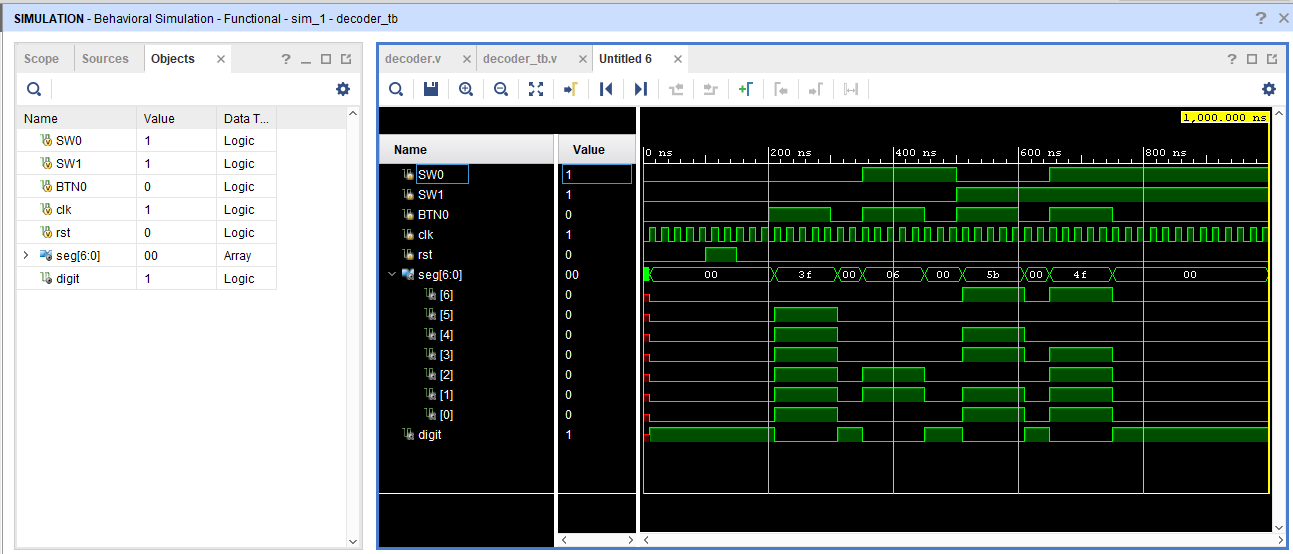
\includegraphics[width=1.0\textwidth ]{01_images/Vivado_lab1_BS.PNG}
	\caption{Vivado behavioral simulation of the decoder module.}
	\label{fig: Vivado_lab1_BS}
\end{figure}


%\subsection{Virtual Machine VM}\label{subsec: Virtual Machine}
%A virtual machine is used to run Ubuntu 18.04 LTS which is supported for five years and is free of charge. The reason to do so is that software can be developed in an environment while then at the end of the project the entire environment can be shipped and not only code. The software used is VMware Player 14.
%
%\begin{description}
%	\item[VM name] RAMI\_RF\_TUNER
%	\item[username] rami
%	\item[password] 1234
%\end{description}
%
%\subsection{Software Tools}\label{subsec: software_tools}
%Used for documentation is 
%\begin{enumerate}[(a)]%for capital roman numbers.
%	\item Git, GitHub
%	\item \LaTeX
%	\item MiK\TeX Consol
%	\item \TeX Studio
%	\item Pandoc \linebreak
%	is used for Markdown to Latex conversion
%	\item Altium Designer v15.1
%\end{enumerate}
%
%\subsection{Git, GitHub}\label{subsec: install_git}
%\href{https://git-scm.com/downloads}{Git} is a fast-version-control tool that  allows the engineer to jump back to any commit that he made. It is available on the three major operating systems Windows, Mac OS X, and Linux/Unix. For Windows there is an additional benefit git comes with a built in Linux/Unix bash terminal so that Linux/Unix commands can be used on Windows and is called Git Bash.
%
%Install Git on Ubuntu 18.04 LTS
%Open the terminal and type Git. If Git is not installed it will show as listing \ref{lst:git install on ubuntu}. Just in case you haven't been working yet with Linux the password is never shown by typing it. After a successful installation the version can be checked.
%\begin{lstlisting}[language=bash,caption={git common commands},label=lst:git install on ubuntu]
%rami@ubuntu:~$ git
%Command 'git' not found, but can be installed with:
%sudo apt install git
%
%rami@ubuntu:~$ sudo apt install git
%[sudo] password for rami: 
%
%rami@ubuntu:~$ git --version
%git version 2.17.1
%
%\end{lstlisting}
%
%Initializing a git repository in an existing folder locale:
%\begin{lstlisting}[language=bash,caption={Initializing a git repository},label=lst: git init]
%    $ git init
%    $ git add README.md
%    $ git commit -m "first commit"
%    $ git remote add origin https://github.com/userName/repositoryName.git
%    $ git push -u origin master
%\end{lstlisting}
%...or cloning an existing repository from GitHub a git repository in an existing folder locale:
%\begin{lstlisting}[language=bash,caption={Clone git repository},label=lst: git clone]
%    $ git clone https://github.com/userName/repositoryName.git
%\end{lstlisting}
%…or push an existing repository from the command line
%\begin{lstlisting}[language=bash,caption={Remote git repository on GitHub},label=lst: git remote]
%    $ git remote add origin https://github.com/haringd/GeocalculatoriOSHW7.git
%    $ git push -u origin master
%\end{lstlisting}
%…or most common git commands used in the command line
%\begin{lstlisting}[language=bash,caption={git common commands},label=lst:git common]
%    $ git pull
%    $ git status
%    $ git add .
%    $ git commit -m "Your commit text"
%    $ git push
%    
%    $ git log
%    $ git checkout <commit>
%\end{lstlisting}
%
%
%
%
%\subsection{Install \LaTeX}\label{subsec: install_latex}
%\subsubsection{Install MiKTeX}\label{subsubsec: install_miktex}
%\href{https://miktex.org/}{MiKTeX} provides package management for \LaTeX that handles most packages used for documentation.  
%
%\subsubsection{Install TexStudio}\label{subsubsec: install_texstudio}
%\href{https://www.texstudio.org/}{TexStudio} is a convenient front end to edit and write \LaTeX syntax. Like most IDEs it provides auto-completion (ctrl + space). It also provides compiler and build system to convert \LaTeX into a PDF format. Furthermore it integrates easy into git which makes it easier to collaborate in a team.
%
%\subsection{TexStudio Hints}\label{subsec: texstudio_hints}
%\subsubsection{Edit Default Language and Dictionary}
%As shown in Figure \ref{fig: texstudio_selectDefaultLanguage}, this can be done under Preferences -> Language Checking.
%
%
%\subsubsection{Convert a *.md file into a *.tex file}
%Pandoc can be used to convert, with a simple terminal command, a *.md file into a *.tex file. Easiest is to convert the file as pre compiler option which can be added shown in Figure \ref{fig: texstudio_convertMDfiletoTEXfilewithPandoc}. The terminal command is shown in Listing \ref{lst: pandoc_bash_convert_file}
%
%\begin{lstlisting}[language=bash, caption=Terminal command that converts .md to .tex files, label=lst: pandoc_bash_convert_file]
%pandoc -f markdown -t latex -o onepage.tex ONEPAGE.md.
%\end{lstlisting}
%
%\begin{figure}[ht]
%	\centering
%	\includegraphics[width=400px ]{01_images/texstudio_convertMDfiletoTEXfilewithPandoc}
%	\caption{Language Settings in TexStudio.}
%	\label{fig: texstudio_convertMDfiletoTEXfilewithPandoc}
%\end{figure}
%
%\subsection{biblatex, make citations with \LaTeX}\label{subsec: Bibtex, make citations with LaTeX}
%In order to run the citation properly use the following commands in bash or windows terminal on the file.
%\begin{verbatim}
%    $ pdflatex reportRFTuner
%    $ biber reportRFTuner
%    $ pdflatex reportRFTuner
%\end{verbatim}
%That solves the problem of not showing the citations after editing the *.bib file correctly.
%
%An easy way to handle citations is to use \href{https://www.mendeley.com}{Mendeley} which allows to copy a citation in bibtex format and simply append it to the *.bib file. Just in case you wonder where you got bibtex from it was installed with miktex or texstudio. 
%
%A bibtex file *.bib has the following syntax and is used with the \\cite{Vizmuller1995} command:
%
%\begin{lstlisting}
%	@book{Vizmuller1995,
%		address = {Boston, London},
%		author = {Vizmuller, Peter},
%		isbn = {0-89006-754-6},
%		mendeley-groups = {RF{\_}TUNER RAMI{\_}2018},
%		pages = {281},
%		publisher = {Artech House, Inc.},
%		title = {{RF Design Guide}},
%		year = {1995}
%	}
%	@misc{key_to_cite_a_webpage_as_example,
%	mendeley-groups = {RF{\_}TUNER RAMI{\_}2018},
%	title = {{Multi-Aperture cores (2867000102) - Fair Rite}},
%	url = {https://www.fair-rite.com/product/multi-aperture-cores-2867000102/},
%	urldate = {2018-07-18}
%	}
%	
%\end{lstlisting}
%
%\subsection{Altium Designer v15.1}\label{subsec: Altium Designer v15.1}
%This is an Altium Designer, short Altium, tutorial that shall guide the user trough the most common steps of Altium.
%
%It is assumed that Altium  is installed on your PC or you have access to it trough the GVSU software of the School of Engineering. 
%
%\begin{enumerate}
%	\item
%Pres Windows key on keyboard and type "Altium" and press enter or double click on Altium Icon, see figure \ref{fig: Altium Icon} on your Desktop if available to start the software package.
%
%\begin{figure}[htbp]
%	\centering
%	\includegraphics[width=0.3\textwidth]{01_images/Altium_Icon.PNG}
%	\caption{Altium Icon.}
%	\label{fig: Altium Icon}
%\end{figure}
%
%\item 
%Altium starts and if no project is open it should look like figure \ref{fig: Altium No Project open}.
%\begin{figure}[H]
%	\centering
%	\includegraphics[width=0.7\textwidth]{01_images/Altium_noProject.PNG}
%	\caption{Altium No Project open.}
%	\label{fig: Altium No Project open}
%\end{figure}
%
%\item
%To start a new project select in menu bar "File" $\rightarrow$ "New" $\rightarrow$ "Project" as shown in figure \ref{fig: Altium new Project}.
%\begin{figure}[H]
%	\centering
%	\includegraphics[width=0.7\textwidth]{01_images/Altium_newProject.PNG}
%	\caption{Altium new Project.}
%	\label{fig: Altium new Project}
%\end{figure}
%
%\item
%The Altium new project dialog appears. Select "PCB Project" in the first column and default in the second one. 
%In the field Name you chose an appropriate project name like "Test1" as example.
%In the field Location you chose an appropriate space to store the project. On your own machine it is beneficial if it is somewhere on the C: drive or on an GVSU blade server on the W: drive. 
%The version control is unchecked as well as the Managed Project.
%If version control is desired the best why to do it, according the authors personal opinion, is to create the project into a git repository and do the version control manually with git in combination with GitHub or GitLab.  \\
%\textbf{Note:} In the naming and location instead of spaces use underscores this avoids unwanted magic errors.   
%\begin{figure}[H]
%	\centering
%	\includegraphics[width=0.7\textwidth]{01_images/Altium_newProjectDialog.PNG}
%	\caption{Altium new Project dialog.}
%	\label{fig: Altium new Project dialog}
%\end{figure}
%
%\item
%The Altium generated now an empty project which appears in the Project view bar on the left side as shown in figure \ref{fig: Altium empty Project}. The project does not contain any documents yet.
%\begin{figure}[H]
%	\centering
%	\includegraphics[width=0.7\textwidth]{01_images/Altium_emptyProject.PNG}
%	\caption{Altium empty Project.}
%	\label{fig: Altium empty Project}
%\end{figure}
%
%\item
%The first thing is to add a schematic sheet which allows to draw a circuit. To add a schematic right click on the empty project $\rightarrow$ Add New to Project $\rightarrow$ Schematic. It is possible to do the same step in menu bar "File" $\rightarrow$ New... $\rightarrow$ Schematic. If the second procedure is used be aware that if you have multiple projects the new schematic sheet will be added to the selected project in project view window.
%\begin{figure}[H]
%	\centering
%	\includegraphics[width=0.7\textwidth]{01_images/Altium_addSchematic.PNG}
%	\caption{Altium add Schematic sheet.}
%	\label{fig: Altium add Schematic}
%\end{figure}
%
%\item
%After a document is generated it is good practice to save it. Chose a expressive name for the sheet, and keep in mind that Altium allows you to build an hierarchical sheet structure with top level and multiple sheets. Furthermore, Altium is a huge software package which results in complexity, so it can crash a lot, save often! The short cut to save is \textbf{CTRL+S}  
%\begin{figure}[H]
%	\centering
%	\includegraphics[width=0.7\textwidth]{01_images/Altium_saveScheet.PNG}
%	\caption{Altium save schematic sheet with an expressive name.}
%	\label{fig: Altium_saveSheet }
%\end{figure}
%
%\item
%In the generated document which is a schematic sheet the Document options have to be set. Right click mostly anywhere on the schematic sheet and  
%\begin{figure}[H]
%	\centering
%	\includegraphics[width=0.7\textwidth]{01_images/Altium_DocumentOptions.PNG}
%	\caption{Altium change options of the generated Document in this case a schematic sheet.}
%	\label{fig: Altium_DocumentOptions }
%\end{figure}
%
%
%\end{enumerate} %ALtium designer
%
%\begin{table}[ht]
%	\begin{center}
%		\begin{tabular}{|| c | c  ||} 
%			\hline
%			Shortcut & Description  \\ 
%			[0.5ex] 
%			\hline\hline
%		
%			\textbf{CTRL+S} & Save selected document \\ \hline
%			\textbf{p} & Press "P" as your mouse is over an open document to open placement options. \\ \hline

%		\end{tabular}
%	\end{center}
%	\caption{$\mu C$ pin occupation}
%\end{table}

\section{Conclusion}\label{sec: Conclusion}
%The lab demonstrates the use of the ipython as simple and fast scripting language that allows access to vast number of packages that allows an decreased development time. The Jupiter Notebook provides a way to program and develop interactive GUIs that allows partially run code in separate cells.
%
 
\section{Appendix} \label{sec: Appendix}
The appendix contains code listening and other large information parts that contain partial or complete relevance to the reports topic. 

\inputencoding{latin1}
\subsection{Python code Listings Part I - RGB LED Driver} \label{subsec: Python code Listings Part I}
\lstinputlisting[style=PythonStyle, language=Python, caption={Jupyter Notebook file \_\_init\_\_ saved as *.py file.}, label=lst: Part1_1] {03_listings/__init__.py }
\lstinputlisting[style=PythonStyle, language=Python, caption={Jupyter Notebook file base saved as *.py file.}, label=lst: Part1_2]{03_listings/base.py }
\lstinputlisting[style=PythonStyle, language=Python, caption={Jupyter Notebook file myrgbled saved as *.py file.}, label=lst: Part1_3] {03_listings/myrgbled.py }
\subsection{Python code Listings Part II - LED Groove Bar} \label{subsec: Python code Listings Part II}
\lstinputlisting[style=PythonStyle, language=Python, caption={Part II - LED Groove Bar Python code.}, label=lst: Python Part 2]{03_listings/LEDBar_Grove.py}
\subsection{Python code Listings Part III - Music Synthesizer} \label{subsec: Python code Listings Part III}
%\lstinputlisting[style=PythonStyle, language=Python, caption={Jupyter Notebook file Rand\_game saved as *.py file.}, label=lst: Python_Rand_game]{03_listings/Rand_game.py }
%
%\subsection{Python code Listings Part III} \label{subsec: Python code Listings Part III}
%\lstinputlisting[style=PythonStyle, language=Python, caption={Jupyter Notebook file LED\_ctrl saved as *.py file.}, label=lst: Python_LED_ctrl]{03_listings/LED_ctrl.py }



\printbibliography
\end{document}          

